\documentclass[otchet]{SCWorks}

\usepackage{preamble}

\begin{document}

\chair{математической кибернетики и компьютерных наук}

\title{Моделирование \\ Вариант 5}

\course{4}

\group{451}

\department{факультета КНиИТ}

\napravlenie{09.03.04 "--- Программная инженерия}

\author{Еремеева Тимура Петровича}

\chtitle{доцент, к.\,ф.-м.\,н.}
\chname{С.\,В.\,Миронов}

\satitle{доцент, к.\,ф.-м.\,н.} %должность, степень, звание
\saname{И.\,Е.\,Тананко}

\term{8}

\date{2025}

\maketitle

\secNumbering
\tableofcontents
\section{Задание 1}
Условие задачи:

Решение задачи (листинг):

Вывод:

\section{Задание 2}
Условие задачи: Построить фазовый портрет системы дифференциальных уравнений 

$$
\left\{\begin{matrix}
 \frac{dx}{dt} = -y - x * (x^{2} + y^{2} - 1) \\
 \frac{dy}{dt} = x - y * (x^{2} + y^{2} - 1)
\end{matrix}\right
$$

Решение задачи (листинг):

\begin{minted}{python}
import numpy as np
from scipy.integrate import solve_ivp
import matplotlib.pyplot as plt

# Определение системы уравнений
def system(t, z):
    x, y = z
    dxdt = -y - x * (x**2 + y**2 - 1)
    dydt = x - y * (x**2 + y**2 - 1)
    return [dxdt, dydt]

# Сетка значений для построения фазового портрета
x = np.linspace(-2, 2, 20)
y = np.linspace(-2, 2, 20)
X, Y = np.meshgrid(x, y)

# Вычисление направлений векторного поля
U = -Y - X * (X**2 + Y**2 - 1)
V = X - Y * (X**2 + Y**2 - 1)

# Нормализация векторов для корректного отображения направлений
magnitude = np.sqrt(U**2 + V**2)
U /= magnitude
V /= magnitude

# Построение фазового портрета
plt.figure(figsize=(10, 8))
plt.quiver(X, Y, U, V, color="blue", alpha=0.8)
plt.title("Фазовый портрет системы", fontsize=14)
plt.xlabel("x", fontsize=12)
plt.ylabel("y", fontsize=12)
plt.axhline(0, color='black', linewidth=0.8, linestyle='--')
plt.axvline(0, color='black', linewidth=0.8, linestyle='--')
plt.grid()
plt.show()
\end{minted}

Вывод:

\begin{figure}[h]
    \centering
    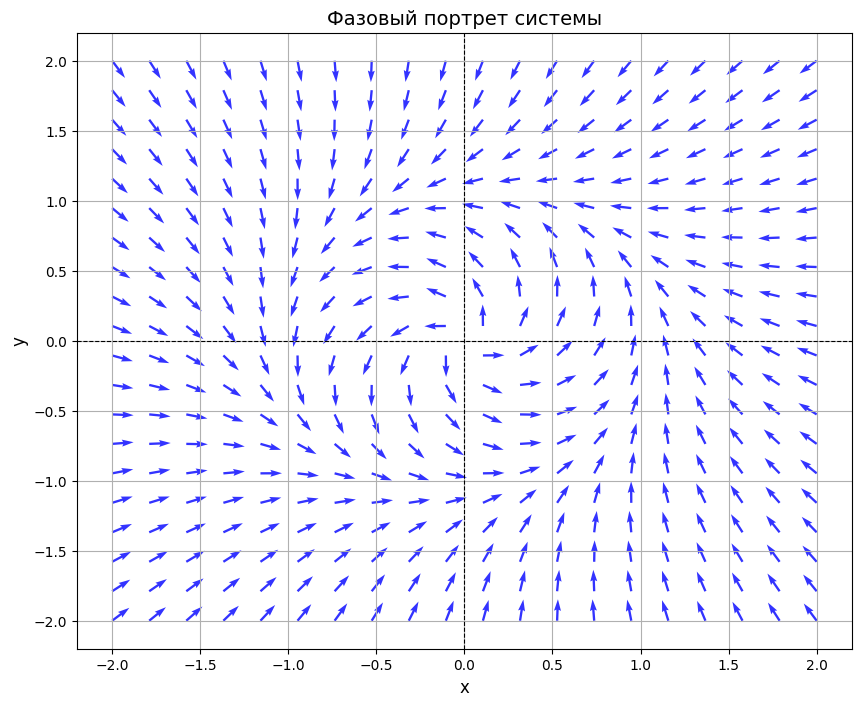
\includegraphics[width=0.8\linewidth]{pics/task2_result.png}
    \caption{Результат работы программы}
    \label{fig:mpr}
\end{figure}
\section{Задание 3}
Условие задачи: Рассмотрим задачу о пьяном прохожем, которую называют еще задачей о случайном блуждании. Предположим, что пьяный, стоя на углу улицы, решает прогуляться. Пусть вероятности того, что, достигнув очередного перекрестка, он пойдет на север, юг, восток или запад, одинаковы. Оценить вероятность того, что, пройдя 10 кварталов, пьяный окажется не далее двух кварталов от места, где он начал прогулку. Оценку вероятности провести на основании 1000 испытаний.

Решение задачи (листинг):

\begin{minted}{python}
import numpy as np
from scipy.integrate import solve_ivp
import matplotlib.pyplot as plt

# Параметры задачи
steps = 10  # Количество шагов
radius = 2  # Радиус от начальной точки
trials = 1000  # Количество испытаний

# Функция для моделирования случайного блуждания
def random_walk(steps):
    """
    Симулирует случайное блуждание.
    """
    # Направления: север (0,1), юг (0,-1), восток (1,0), запад (-1,0)
    directions = [(0, 1), (0, -1), (1, 0), (-1, 0)]
    position = np.array([0, 0])
    for _ in range(steps):
        step = directions[np.random.choice(4)]
        position += step
    return position

# Моделирование и подсчет успешных случаев
success_count = 0
for _ in range(trials):
    final_position = random_walk(steps)
    distance = np.linalg.norm(final_position, ord=2)  # Евклидово расстояние
    if distance <= radius:
        success_count += 1

# Оценка вероятности
probability = success_count / trials

# Вывод результата
print(f"Вероятность того, что пьяный окажется не далее двух кварталов: {probability:.4f}")
\end{minted}

Вывод:

\section{Задание 4}
Условие задачи: Оценить интеграл $I = \int^{\pi}_{0}\sin{x*dx}$ (как показывают элементарные вычисления ), используя метод статистических испытаний, при объемах выборки $n = 10, 20, 50, 100, 1000, 10000$.

Решение задачи (листинг):

\begin{minted}{python}
import numpy as np
from scipy.integrate import solve_ivp
import matplotlib.pyplot as plt

# Функция, подлежащая интегрированию
def f(x):
    return np.sin(x)

# Пределы интегрирования
a, b = 0, np.pi

# Объемы выборки для метода Монте-Карло
sample_sizes = [10, 20, 50, 100, 1000, 10000]

# Вычисление интеграла методом Монте-Карло
results = []
for n in sample_sizes:
    # Генерация случайных точек в пределах интегрирования
    x_samples = np.random.uniform(a, b, n)
    # Оценка интеграла
    integral_estimate = (b - a) * np.mean(f(x_samples))
    results.append((n, integral_estimate))

# Вывод результатов
print("Результаты вычисления интеграла методом Монте-Карло:")
for n, estimate in results:
    print(f"n = {n}: I ≈ {estimate:.6f}")
\end{minted}

Вывод:

\section{Задание 5}
Условие задачи: Случайные величины $X$ и $Y$ независимы и имеют нормальное распределение с математическим ожиданием $0$ и дисперсией $1$. Оценить $P(|X-Y|<=1)$ на основании $1000$ выборочных значений пар $(x_{i}, y_{i})$, $i=1,...,1000$.

Решение задачи (листинг):

\begin{minted}{python}
import numpy as np
from scipy.integrate import solve_ivp
import matplotlib.pyplot as plt

# Параметры нормального распределения
mean = 0
std_dev = 1

# Количество выборочных значений
n_samples = 1000

# Генерация выборок для X и Y
X = np.random.normal(mean, std_dev, n_samples)
Y = np.random.normal(mean, std_dev, n_samples)

# Вычисление |X - Y| и подсчет случаев, удовлетворяющих условию
absolute_differences = np.abs(X - Y)
success_count = np.sum(absolute_differences <= 1)

# Оценка вероятности
probability_estimate = success_count / n_samples

# Вывод результата
print(f"Оценка вероятности P(|X - Y| <= 1): {probability_estimate:.4f}")
\end{minted}

Вывод:

\section{Задание 6}
Условие задачи: Пусть в течение суток длительность интервала времени между очередными поступлениями трамваев на остановку распределена экспоненциально с математическим ожиданием равным 15 минутам. Один раз в сутки пассажир приходит на остановку в случайный момент времени суток (равномерное распределение длительности) и ожидает очередной трамвай в течение времени $\Delta$. Провести 1000 испытаний с моделью и оценить математическое ожидание $\Delta$.

Решение задачи (листинг):

\begin{minted}{python}
import numpy as np

# Параметры задачи
mean_interval = 15  # Средний интервал между трамваями (в минутах)
rate = 1 / mean_interval  # Параметр экспоненциального распределения
n_trials = 1000  # Количество испытаний

# Симуляция
waiting_times = []
for _ in range(n_trials):
    # Момент прихода пассажира (в минутах с начала суток)
    passenger_arrival = np.random.uniform(0, 1440)  # 1440 минут в сутках
    # Генерация интервалов между трамваями в течение суток
    tram_arrivals = [0]
    while tram_arrivals[-1] < 1440:
        tram_arrivals.append(tram_arrivals[-1] + np.random.exponential(scale=mean_interval))
    # Удаляем последний элемент, если он больше 1440 минут
    tram_arrivals = np.array(tram_arrivals[:-1])
    # Проверка на наличие следующего трамвая
    next_trams = tram_arrivals[tram_arrivals >= passenger_arrival]
    if next_trams.size == 0:  # Если массив пуст, возвращаемся к первому трамваю следующего дня
        waiting_time = 1440 - passenger_arrival + tram_arrivals[0]
    else:
        waiting_time = next_trams.min() - passenger_arrival
    waiting_times.append(waiting_time)

# Оценка математического ожидания времени ожидания
expected_waiting_time = np.mean(waiting_times)
# Вывод результата
print(f"Оценка математического ожидания времени ожидания (\u0394): {expected_waiting_time:.2f} минут")
\end{minted}

Вывод:
\begin{minted}{shell}
    ценка математического ожидания времени ожидания (Δ): 14.99 минут
\end{minted}

\end{document}